\section{S4 -- Urządzenia sieci komputerowych}

Sieci komputerowe zbudowano, aby wymieniać dane między komputerami. Wymianę tą zapewnia zastosowanie odpowiedniego sprzętu oraz oprogramowania. Podstawowymi urządzeniami stosowanymi do budowy sieci komputerowych są:

\begin{itemize}
	\setlength\itemsep{1pt}
	\item \textbf{Modem} (ang. \textit{Modulator DEModulator}) to urządzenie, które zamienia cyfrowe dane, generowane przez komputer, na sygnały analogowe i wysyła je za pomocą sieci. Podczas odbierania danych z sieci sygnały analogowe są zamieniane na cyfrowe i przekazywane do komputera. Modem może być wykorzystywany do połączenia komputera lub sieci LAN z Internetem za pośrednictwem stacjonarnej linii telefonicznej lub do przesyłania danych pomiędzy sieciami LAN. Zaletą modemu jest powszechna dostępność do usługi. Modemy są stosowane również w sieciach telewizji kablowej i telefonii komórkowej (np. modemy 3G/4G).

	\item \textbf{Karta sieciowa} (\textit{Network Interface Card}) to urządzenie łączące komputer z lokalną sie­cią komputerową. Głównym zadaniem karty sieciowej jest przekształcanie ramek danych w sygnały, które są przesyłane w sieci komputerowej. Karta sieciowa w standardzie \textbf{Ethernet} (najczęściej spotykanym) ma unikatowy w skali światowej \textbf{adres fizyczny MAC} (ang. \textit{MAC adress}), przyporządkowany jej podczas produkcji i zapisany w pamięci ROM. Karty mogą pracować z różnymi prędkościami. Obecnie standardem w przypadku sieci przewodowych są karty sieciowe pracujące z prędkością 100 Mb/s lub 1 Gb/s. W bezprzewodowych kartach sieciowych do przesyłania danych wykorzystywane są fale radiowe. Karta sieciowa może być wlutowana w płytę główną komputera lub innego urządzenia, albo montowana w różnych odmianach złączy PCI, PCMCIA, ExpressCard, USB, PCIExpress.

	\item \textbf{Wzmacniacz} (ang. \textit{repeater}), zwany również regeneratorem, wykorzystuje się w miejscach, w których jest wymagane wzmocnienie lub regeneracja sygnału, niezbędne do zwiększenia zasięgu sieci. Rzadko jest to samodzielne urządzenie. Najczęściej funkcję wzmacniaka pełni urządzenie sieciowe posiadające własne zasilanie w energię elektryczną, np. koncentrator.

	\item \textbf{Koncentrator} (ang. \textit{hub}) to urządzenie posiadające wiele portów służących do przyłączania stacji roboczych lub innych urządzeń. Koncentratory mogą być pasywne i aktywne. Pasywny pełni tylko funkcję skrzynki łączeniowej, rozsyłającej sygnał otrzymany na jednym porcie do wszystkich pozostałych. Aktywny dodatkowo wzmacnia sygnały. \textbf{Tworzy domenę kolizyjną}.

	\item \textbf{Most} (ang. \textit{bridge}) to urządzenie posiadające dwa porty, służące do łączenia segmentów sieci. W swojej pamięci zapamiętuje adresy MAC urządzeń przyłączonych do poszczególnych portów. Po otrzymaniu ramki danych sprawdza adres miejsca docelowego i określa, do jakiego segmentu należy przesłać daną ramkę. Gdy komputer z jednego segmentu wysyła wiadomość, most analizuje zawarte w niej adresy MAC i na tej podstawie podejmuje decyzję, czy sygnał przesłać do drugiego segmentu, czy go zablokować. W sieci nie są wtedy przesyłane zbędne ramki, dzięki czemu zwiększa się jej wydajność.

	\item \textbf{Punkt dostępowy} (ang. \textit{Access Point}) to urządzenie zapewniające stacjom bezprzewodowym dostęp do zasobów sieci za pomocą bezprzewodowego medium transmisyjnego. Pełni funkcję mostu łączącego sieć bezprzewodową z siecią przewodową. Do sieci bezprzewodowych są przyłączane laptopy, palmtopy, smartfony oraz komputery stacjonarne wyposażone w karty bezprzewodowe. Punkt dostępowy może być połączony w jedno urządzenie z routerem.

	\item \textbf{Przełącznik} (ang. \textit{switch}) oferuje te same funkcje, co koncentrator, a dodatkowo pozwala, podobnie jak most, podzielić sieć na segmenty. Urządzenie posiada wiele portów przyłączeniowych, pozwalających na podłączenie komputerów, innych przełączników lub koncentratorów. Porty w przełączniku mogą pracować z jednakowymi prędkościami (przełączniki symetryczne) lub z różnymi prędkościami (przełączniki asymetryczne). Przełączniki mogą być wyposażone w funkcje zarządzania i monitoringu sieci. W odróżnieniu do huba \textbf{nie tworzy domeny kolizyjnej}.

	\item \textbf{Router} to urządzenie stosowane do łączenia sieci, np. do przyłączania sieci LAN do Internetu. Jest urządzeniem konfigurowalnym, pozwala sterować przepustowością sieci i podnosi jej bezpieczeństwo.

	\item \textbf{Brama sieciowa} (ang. \textit{gateway}) to urządzenie, za pośrednictwem którego komputery z sieci lokalnej komunikują się z komputerami w innych sieciach. W sieci TCP/IP domyślna brama oznacza router, do którego komputery sieci lokalnej mają wysyłać pakiety adresowane do innej sieci, np. internet. Niektóre bramy umożliwiają komunikację między sieciami, w których działają różne protokoły.

	\item \textbf{Bramka VolP} (ang. \textit{Voice over Internet Protocol}) to urządzenie, którego zadaniem jest umożliwienie wykonywania połączeń telefonicznych tradycyjnym aparatem telefonicznym za pośrednictwem sieci komputerowej wykorzystującej protokół IP. Bramka VoIP zamienia analogowy sygnał mowy oraz sygnały wybierania numeru telefonicznego na sygnały VoIP.

	\item \textbf{Zapora sieciowa} (ang. \textit{firewall}) to dedykowany sprzęt komputerowy wraz ze specjalnym oprogramowaniem, blokujący niepowołany dostęp do sieci. Jego zadaniem jest filtrowanie połączeń wchodzących (ochrona przed nieuprawnionym dostępem z zewnątrz) i wychodzących do sieci (ochrona przed nieuprawnionym wypływem danych z sieci lokalnej na zewnątrz). Rolę zapory może pełnić również komputer wyposażony w system operacyjny, np. Linux z odpowiednim oprogramowaniem.
\end{itemize}

Urządzenia sieciowe mogą być ze sobą łączone, np. router z przełącznikiem i punk­tem dostępowym, zintegrowana brama sieciowa zawierająca router, przełącznik, firewall, bramkę VoIP i punkt dostępowy.

\textbf{Domena kolizyjna}

\begin{figure}[H]
	\centering
	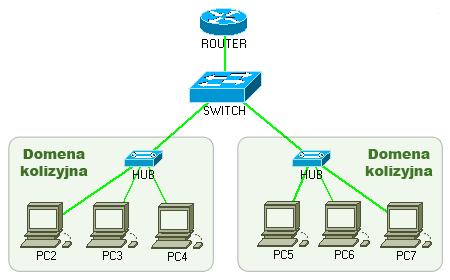
\includegraphics[scale=0.5]{s4_domena_kolizyjna.png}
	\caption{Domena kolizyjna}
\end{figure}

Jeżeli poprzez jedno medium transmisyjne (kabel) co najmniej dwa urządzenia transmitują dane może dojść do kolizji. Kolizje są zjawiskiem niepożądanym – powodują, iż żadna z wysłanych w tym momencie informacji nie dotrze do adresata. Jednak kolizji w sieciach, w których dostęp do nośnika przyznawany jest na zasadzie rywalizacji, nie da się uniknąć. Obszar sieci, w którym może dojść do kolizji nazywamy domeną kolizyjną. Możemy zmniejszać ryzyko kolizji odpowiednio projektując sieć komputerową. Należy również pamiętać, iż maksymalna ilość urządzeń w domenie kolizyjnej wynosi 1024. Przy czym im więcej urządzeń, tym większe prawdopodobieństwo wystąpienia kolizji. Domenę kolizyjną ograniczają urządzenia pracujące w warstwach wyższych niż pierwsza modelu OSI. Tym samym koncentratory i huby będą wewnątrz domeny kolizyjnej, a switch (przełącznik) czy router będą ją ograniczać.

\textbf{Domena rozgłoszeniowa}

\begin{figure}[H]
	\centering
	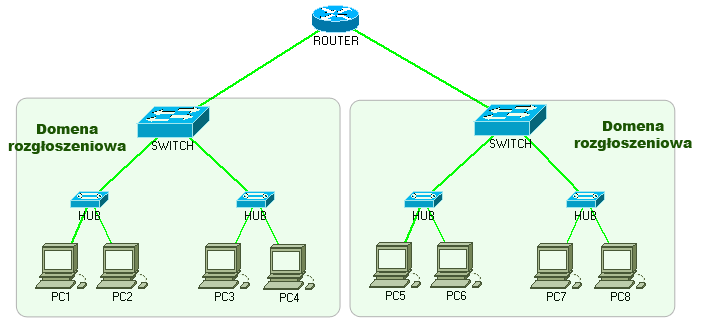
\includegraphics[scale=0.5]{s4_domena_rozgloszeniowa.png}
	\caption{Domena rozgłoszeniowa}
\end{figure}

Domena rozgłoszeniowa to taki obszar sieci, do którego dotrze informacja wysyłana przez jedno urządzenie do wszystkich innych – broadcast. Ruch rozgłoszeniowy jest przekazywany poprzez urządzenia pierwszej i drugiej warstwy modelu OSI, tj. koncentratory, huby, mosty czy switche. One zwiększają obszar domeny rozgłoszeniowej. Ograniczają go natomiast urządzenia trzeciej warstwy – routery. Można również utworzyć sieć wirtualną VLAN (sieć komputerowa wydzielona logicznie w ramach innej, większej sieci fizycznej ), która również ograniczy obszar domeny rozgłoszeniowej.

